\chapter{Estado del Arte\label{sec:EstadoDelArte}}

Con el paso del tiempo se ha demostrado que una de nuestras mayores virtudes como seres humanos es la habilidad de aprovechar el saber cultivado por otras personas para realizar nuevos descubrimientos con mayor facilidad. En la actualidad, con la ayuda de Internet esta ventaja se ha visto potenciada hasta límites insospechados.

Como se ha mencionado con anterioridad en el capítulo \ref{sec:introduccion}, a lo largo de los años se han desarrollado numerosas alternativas a los dispositivos presentes en los hospitales y laboratorios utilizados normalmente para el estudio del cerebro. 
\\Aunque se han invertido muchos recursos en estos dispositivos, el objetivo es permitir ampliar el número de personas capaces de estudiar el cerebro humano, consiguiendo  así aumentar las posibilidades de mejorar nuestro conocimiento sobre el mismo.

De esta forma debería ser más fácil realizar nuevos descubrimientos como, por ejemplo, nuevas formas de diagnosticar enfermedades o de realizar una comunicación hombre-máquina para aquellas personas que por algún tipo de discapacidad física o mental no puedan utilizar los medios convencionales.

\clearpage

\section{Dispositivos similares\label{sec:Disp_similares}}

A lo largo de este \textbf{capítulo} se presentarán algunos de los \textbf{dispositivos capaces de capturar un \acrshort{EEG}}, a nivel personal, enfocados a la docencia o, por supuesto, diseñados con el fin de realizar un producto final que vender a terceros.

\subsection{Proyectos personales\label{sec:Pro_personales}}

En internet se pueden encontrar algunos ejemplos de personas que han dedicado su tiempo a crear dispositivos capaces de captar un \acrshort{EEG}. 

\subsubsection{Instructables}

La página web \textbf{instructables.com} ha propuesto a sus usuarios la creación de un sistema de adquisición de \acrshort{EEG} y \acrshort{ECG} sencillo y barato. El dispositivo final resulta muy interesante, pues con unas pocas resistencias, condensadores y un par de amplificadores operacionales son capaces de montar un dispositivo funcional. La figura \ref{} muestra el esquemático final del dispositivo.

\begin{figure} [h]
    \centering
    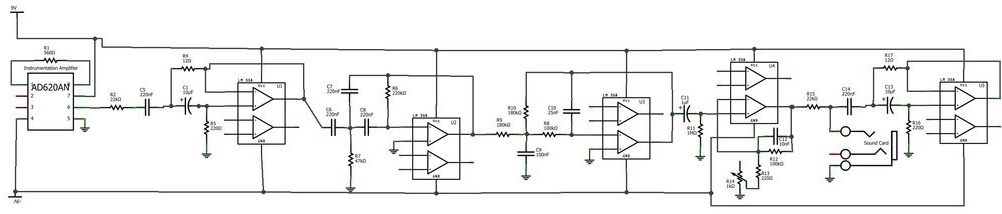
\includegraphics[width=13cm]{EdA_EEG_0}
    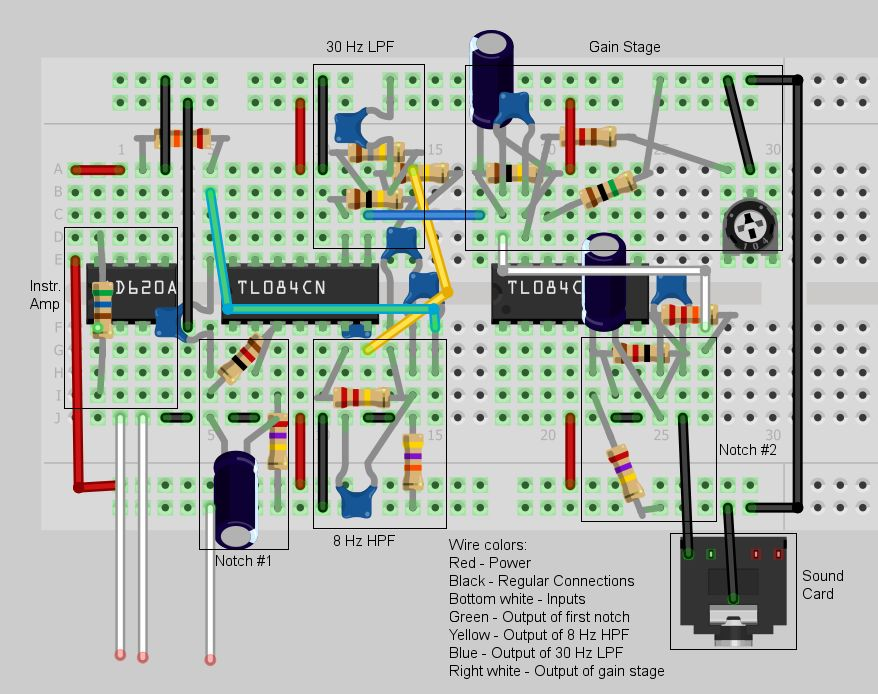
\includegraphics[width=6cm]{EdA_EEG_1}
    \caption{Esquema electrónico casero para la captura de un EEG \cite{DIY_EEG}}
    \label{fig:EdA_EEG_1}
\end{figure}

Este sistema es muy interesante y para fines educativos cumple perfectamente su función pero tiene en cuenta el ruido que afecta a la señal ni otras características importantes como son el aislamiento del paciente de la red eléctrica.

En su página web no especifican el coste total del proyecto pero en base al número de componentes se estima que el coste final es de 60€.

\subsubsection{OpenEEG}

OpenEEG es un proyecto de software libre que pone a disposición de cualquiera que lo necesite un conjunto de herramientas, software y esquemáticos que permiten crear un sistema de adquisición \acrshort{EEG} utilizando una base que se encuentra en continuo desarrollo.

A lo largo de Internet se pueden encontrar un gran número de pruebas de concepto y prototipos basados en este proyecto. En general muestran los resultados obtenidos pero hay algunos que además guían a los más curiosos que se atrevan a intentar construirse uno. Este es el caso de la web http://openeeg.sourceforge.net/buildeeg/ (aún en construcción), donde un usuario anónimo muestra sus resultados y anima a cualquiera con conocimientos básicos de electrónica a intentar repetir el proceso, proporcionando esquemáticos, consejos y software.

El resultado final de este proyecto es el que se muestra en la figura \ref{fig:OpenEEG}.

\begin{figure}[h]
  \centering
  \begin{subfigure}[b]{6.5cm}
   	\centering
    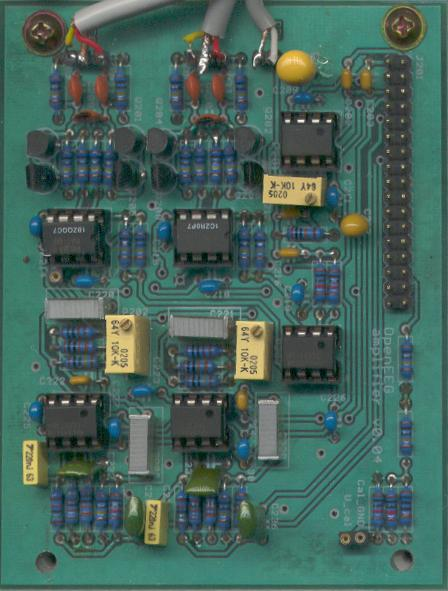
\includegraphics[width=6cm]{Openeeg_amp_l}
    \caption{Tarjeta de adquisición}
    \label{fig:Openeeg_amp_l}
  \end{subfigure}
%  \hfill
  \begin{subfigure}[b]{6.5cm}
  	\centering
    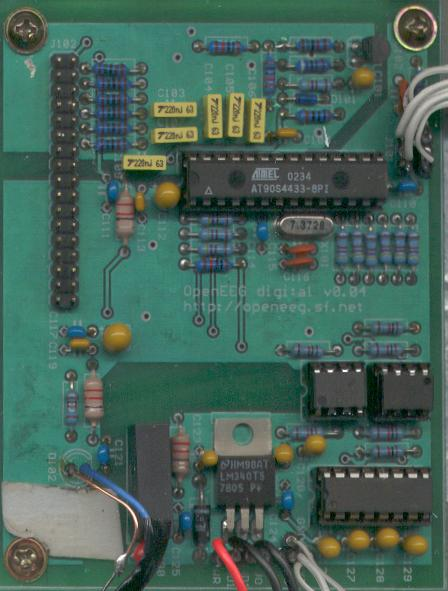
\includegraphics[width=6cm]{openeeg_digital_l}
    \caption{Tarjeta de procesado}
    \label{fig:openeeg_digital_l}
  \end{subfigure}
  \caption{Elementos que conforman OpenEEG \cite{OpenEEG}}
  \label{fig:OpenEEG}
\end{figure}

El sistema está dividido en dos placas principales, una de adquisición encargada del acondicionamiento de la señal mediante resistencias, condensadores y amplificadores operacionales y otra de procesado donde el núcleo es un microcontrolador de ATMEL (presentes también en Arduino). 

Resulta evidente que este proyecto presenta un acabado más profesional ya que tiene en cuenta factores muy importantes como el a acondicionado de la señal para minimizar el ruido y el aislamiento de la alimentación del paciente.

El precio total estimado de este sistema es de 180€ aproximadamente.

\subsubsection{Beanie}

Esta curiosa iniciativa utiliza un analizador de \acrshort{EEG} acoplado a un gorro para que este se ilumine en función del estado y concentración de la persona.

\begin{figure} [h]
    \centering
    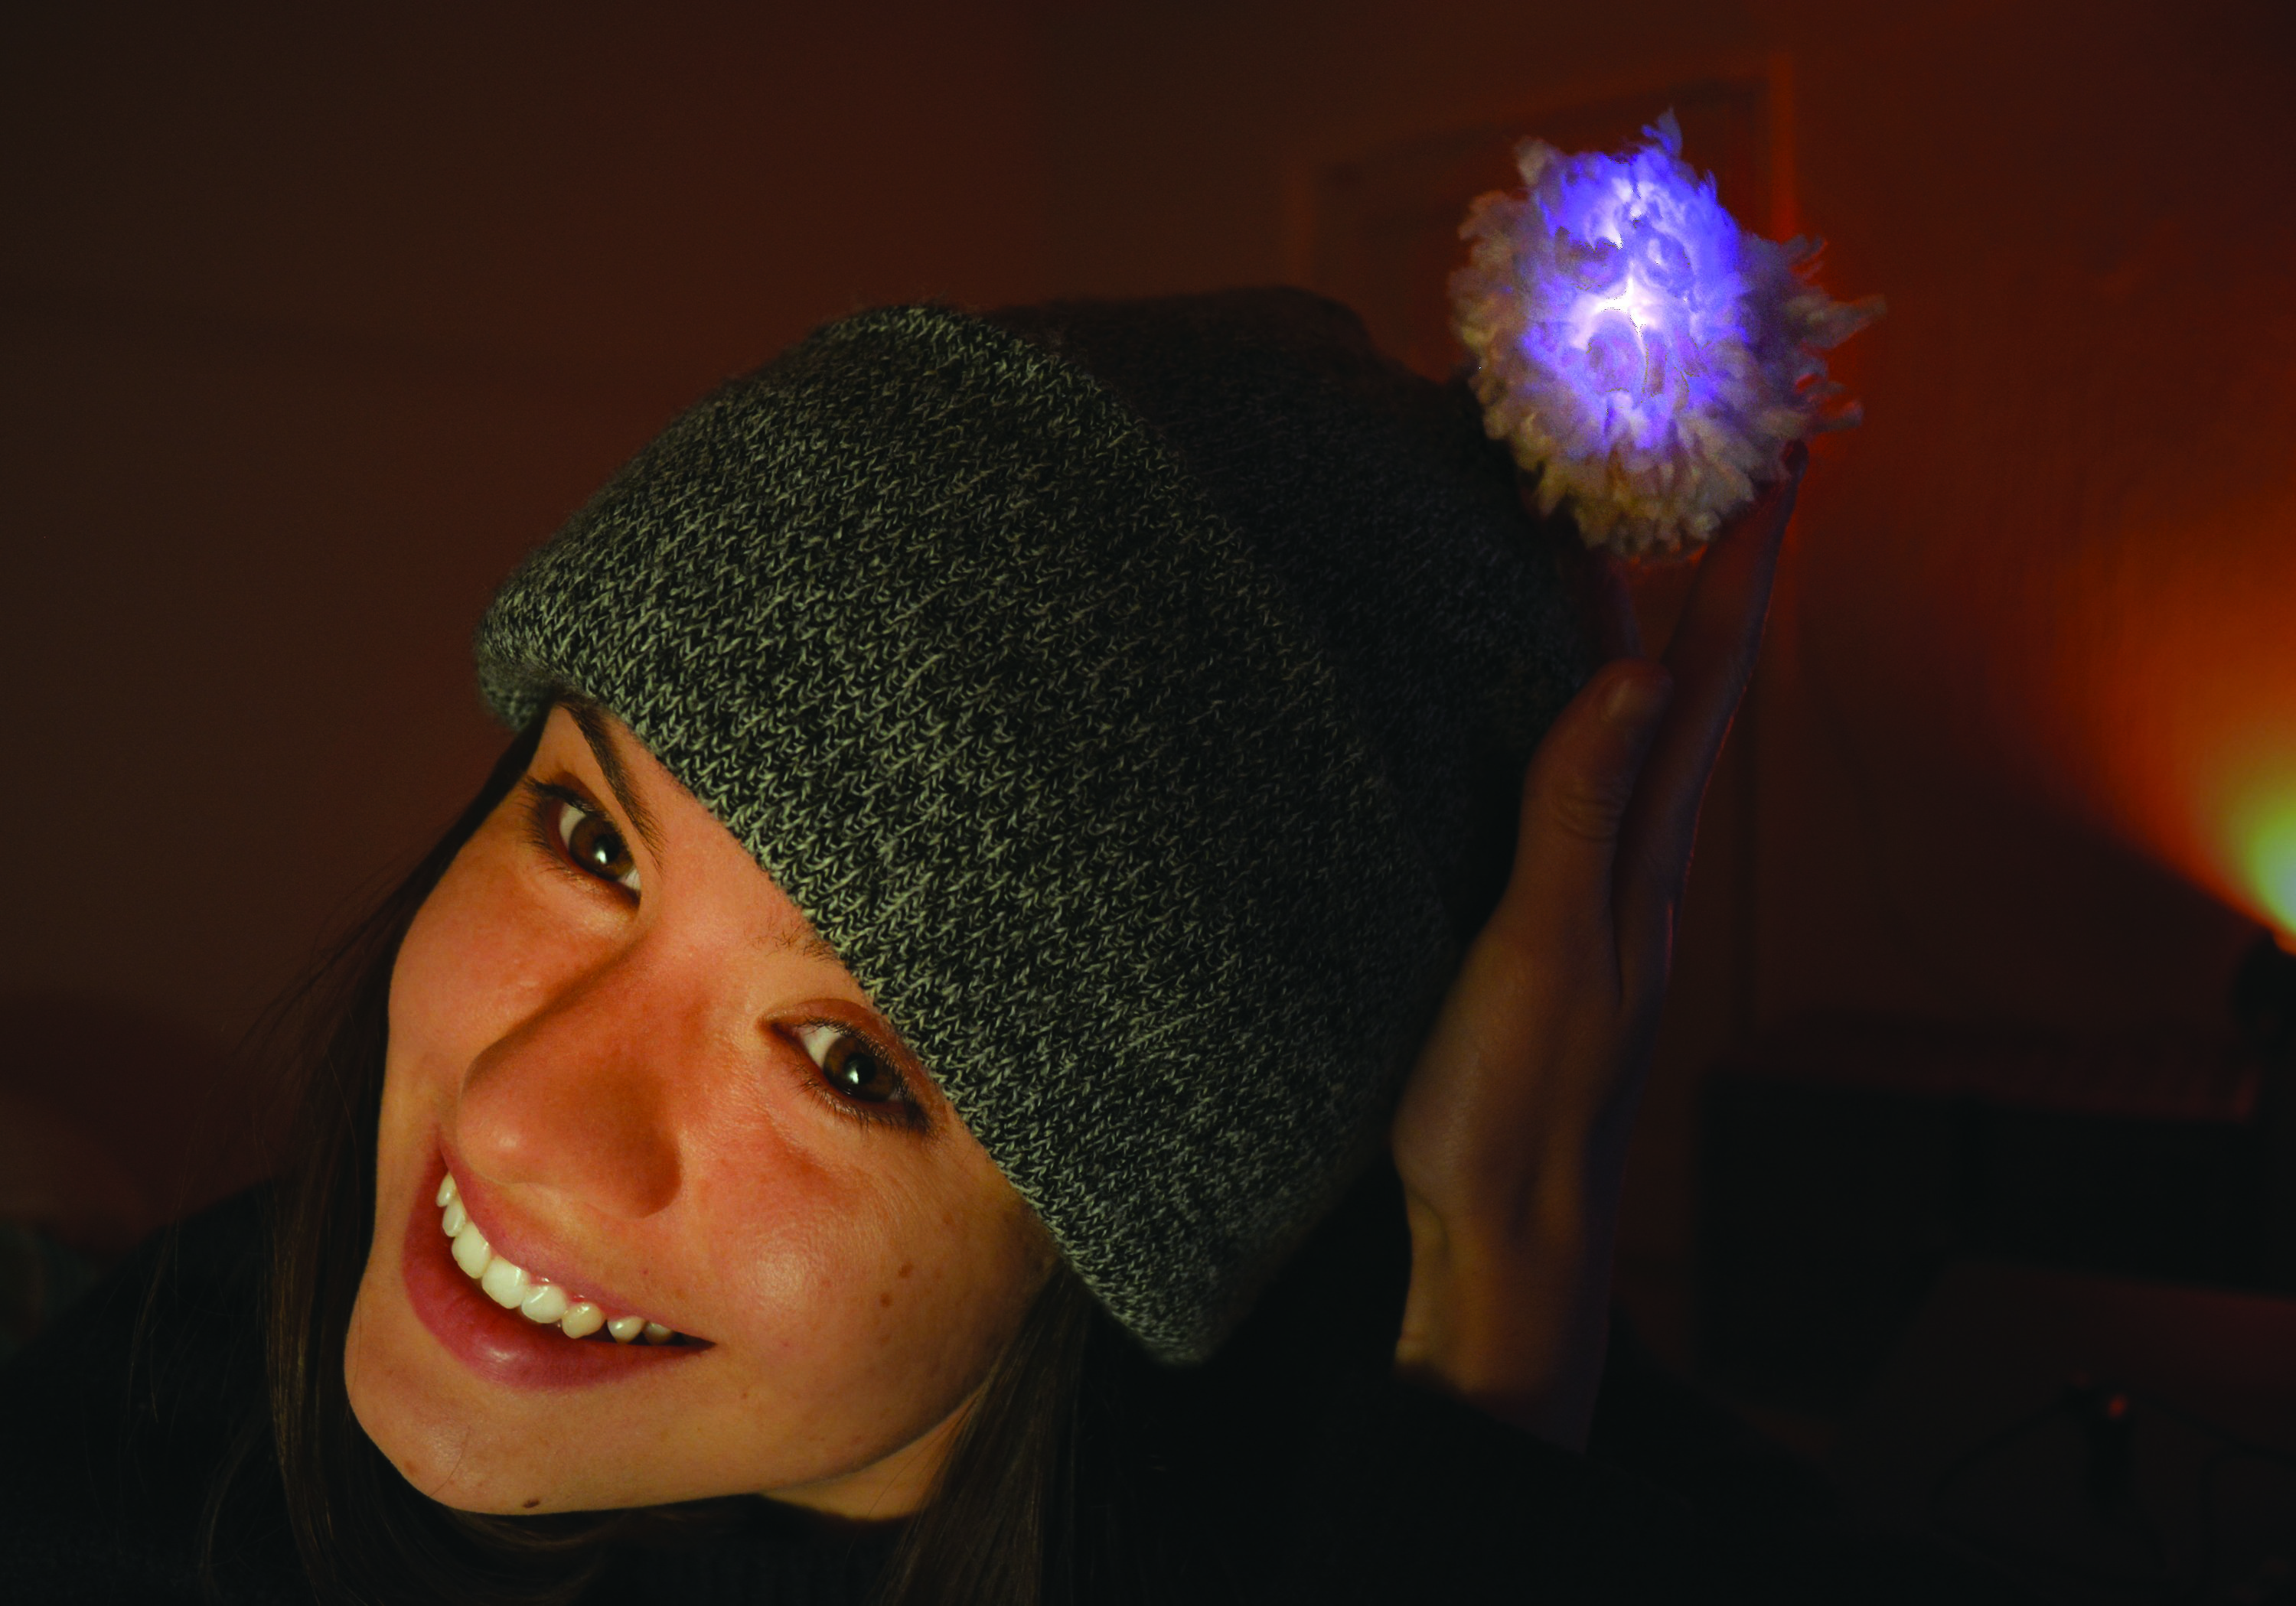
\includegraphics[width=7cm]{EdA_Beanie}
    \caption{Beanie en funcionamiento \cite{beanie}}
    \label{fig:EdA_Beanie}
\end{figure}

El funcionamiento es muy similar al resto de dispositivos ya explicados: se adquieren señales desde electrodos situados en la cabeza, se filtra la señal para eliminar el ruido y se presenta al usuario.

Para la adquisición de la señal utiliza un chip de la compañía Neurosky llamado ThinkGear ASIC Module que tiene integrado un sistema de adquisición y filtrado de señales. Posteriormente está se transfiere a un módulo TinyLily de Arduino que se encargará de realizar un segundo procesado para iluminar el pompón del gorro de la forma deseada.

El dispositivo se monta con relativa facilidad (1-2 días) y su precio ronda los 130€.

\subsubsection{GitHub}

Por último es importante destacar la presencia de GitHub. Esta plataforma permite que la gente suba una gran cantidad de proyectos que normalmente están accesibles.

Aunque los proyectos encontrados no suelen contener información acerca del diseño de placas y el precio final, sí que incluyen una gran cantidad de código que será utilizado como referencia para la implementación del código de este proyecto. Se incluye en la bibliografía algunas de los repositorios de mayor interés.

\subsection{Proyectos docentes\label{sec:Pro_docentes}}

Los proyectos llevados a cabo por universidades y otras instituciones centradas en el estudio y la docencia suelen ser de difícil acceso, pues la documentación generada tras un proyecto se suele aprovechar para realizar publicaciones en las revistas científicas más conocidas.

Sin embargo, en ocasiones los Trabajos Fin de Carrera abordan temas similares y estos si que se encuentran disponibles para cualquiera que tenga acceso a Internet. 

Un ejemplo de esta situación es el Trabajo Fin de Máster de la alumna Nerea Urrestarazu. En este se aborda la creación de un sistema de adquisición de \acrshort{EEG} haciendo uso de un convertidor analógico-digital y un ordenador. Este proyecto se ha utilizado como base para construir otro que mejore sus prestaciones, así que sus características serán ampliadas en posteriores capítulos.

El coste final del proyecto contando sólo los materiales asciende a 100€ aproximadamente.

\subsection{Sistemas comerciales\label{sec:Pro_empresa}}

Muchas empresas han visto este campo como una oportunidad de negocio y han desarrollado varias aplicaciones que hacen uso de la medida de \acrshort{EEG} para diversos propósitos.

\subsubsection{The XWave Headset}

Este sistema es exclusivo de usuarios de iPhone. Por el momento incluye una diadema que, mediante el contacto con la frente, permite ver al usuario sus ondas cerebrales y controlar ciertas aplicaciones.

\begin{figure} [h]
    \centering
    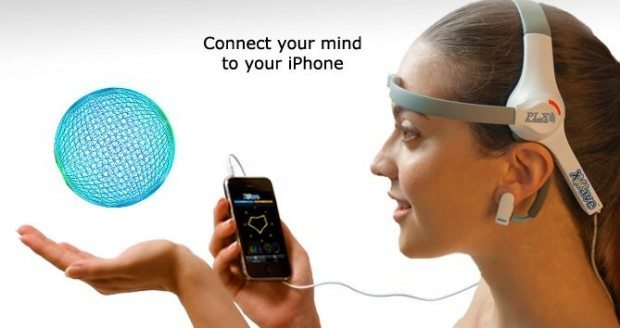
\includegraphics[width=10cm]{xwave}
    \caption{Imagen promocionando el producto}
    \label{fig:xwave}
\end{figure}

El estudio que realiza del \acrshort{EEG} no es muy exhaustivo de modo que no es un candidato a utilizar para estudios médicos pero sí que permite a los usuarios familiarizarse con la terminología y acostumbrarse a dispositivos similares.

Su precio es de 99.90\$, (86€).

\subsubsection{NeuroSky}

Esta compañía ha creado una diadema similar a la presentada con anterioridad. Esta compañía pone a disposición del usuario un paquete de inicio que incluye la diadema, software y una guía de inicio. Este software contiene entre otras aplicaciones una película cuya trama cambia en función del estado mental del usuario

\begin{figure} [h]
    \centering
    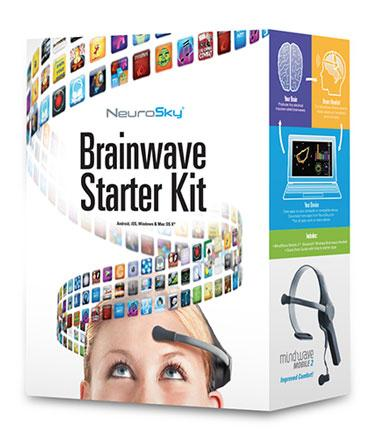
\includegraphics[width=5cm]{MindWave-StarterKit}
    \caption{CAPTION}
    \label{fig:MindWave-StarterKit}
\end{figure}

El precio comercial es de 99.99\$ (86€).

\subsubsection{OpenBCI}

Los ejemplos anteriores tienen características muy interesantes pero ambos son poco adecuados para realizar estudios médicos de las ondas cerebrales. Siguiendo esta premisa se ha creado un proyecto denominado OpenBCI con una extensa comunidad de desarrolladores.

\begin{figure} [H]
    \centering
    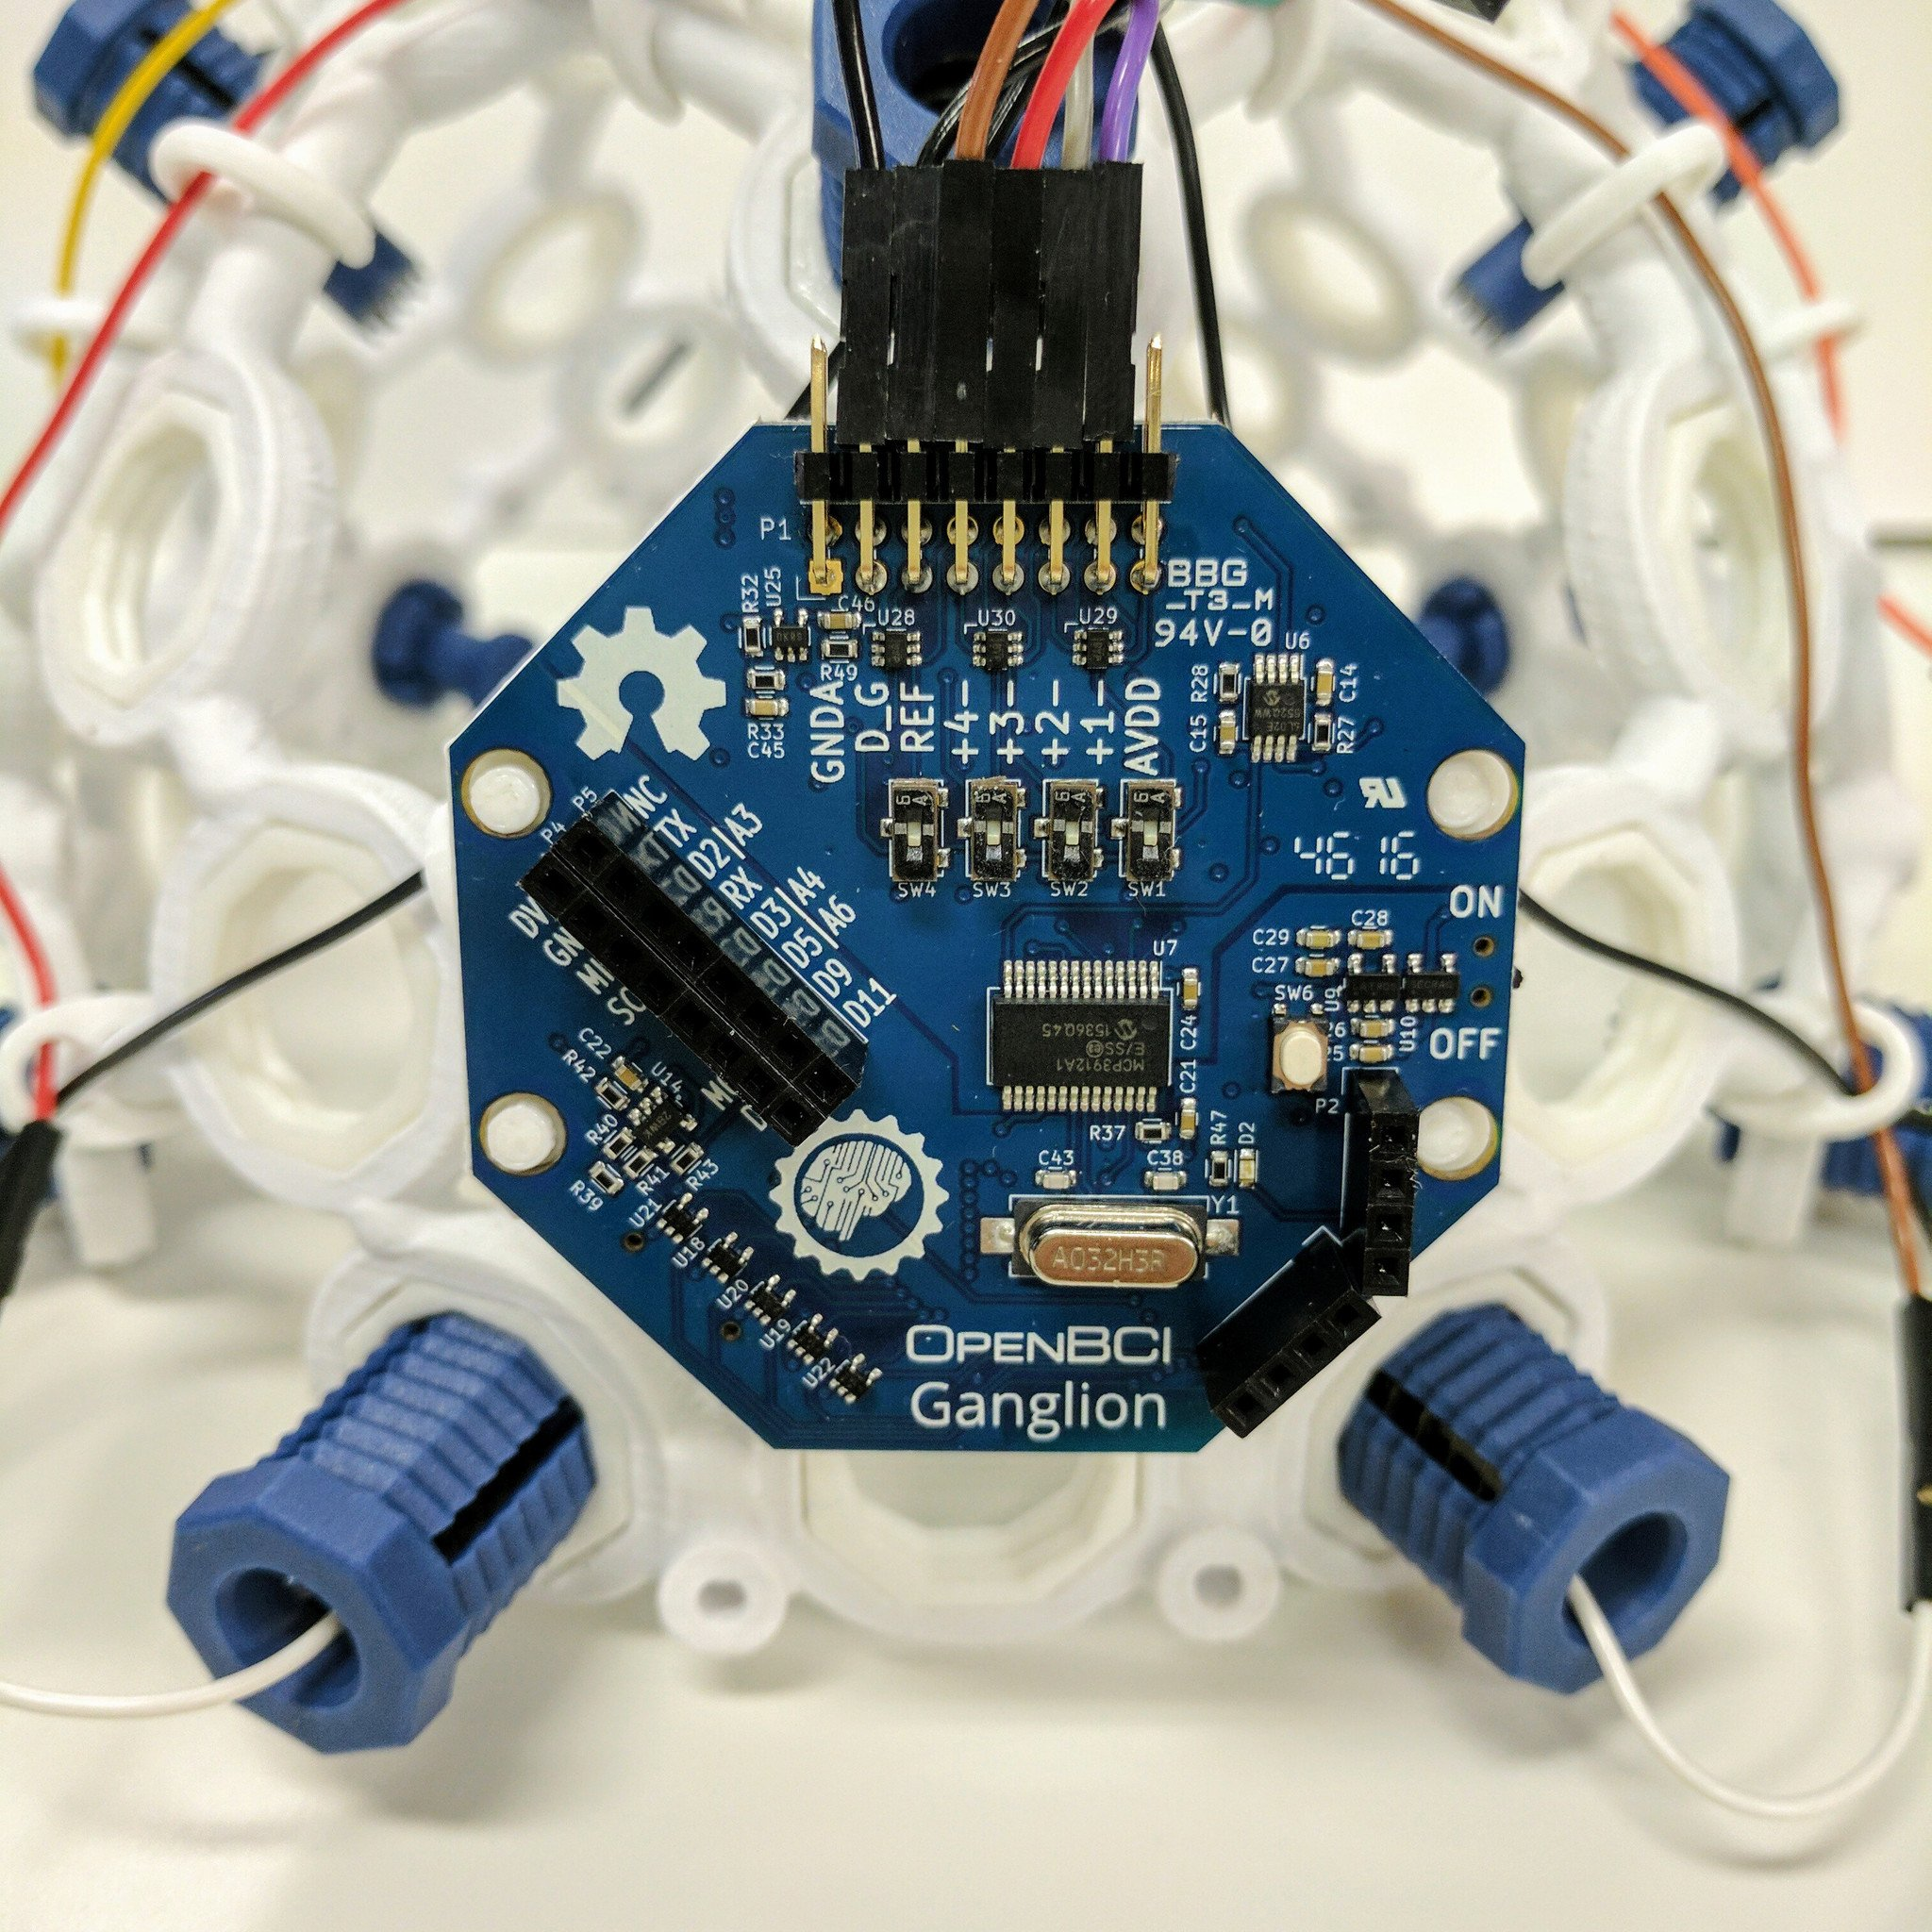
\includegraphics[width=7cm]{GANGLION-mounted}
    \caption{Módulo Ganglion montado sobre un casco \cite{OpenBCI}}
    \label{fig:GANGLION-mounted}
\end{figure}

Este sistema hace uso del convertidor analógico ADS1299 para realizar una adquisición de las señales procedentes del cerebro usando 4 canales. A continuación realiza un procesado inicial y las transmite a un ordenador, donde serán filtradas y reprocesadas para extraer la información de interés.

Está basado en la utilización de módulos, siendo necesario comprar el módulo base (Ganglion) por 200\$ (175€) para funcionar mientras que el resto de módulos son opcionales y son usados para aumentar sus funcionalidades.

\section{Comparativa\label{sec:EdA_comparativa}}

Las mayoría de las alternativas comerciales presentadas a lo largo de este capítulo intentan maximizar el confort del usuario aunque esto afecte al rendimiento del dispositivo. 

Los sistemas orientados a la investigación se centran en los resultados mientras dejan el confort en segundo plano. Por supuesto intentan que el dispositivo sea lo más cómodo posible pero no permiten que esto afecte a las señales medidas.

La tabla \ref{tab:EdA_Comparativa} hace una comparativa de los equipos anteriormente expuestos

\begin{table} [H]
\centering
\begin{tabular}{|c|c|c|}
\hline
\multirow{2}{*}{Dispositivo} 	& Apto para la investigación / 	& \multirow{2}{*}{Precio[€]} \\
 								& Aplicable a la medicina 		&  \\
\hline
Instructables & Sí\footnotemark{} & 60 \\
\hline
OpenEEG & Sí & 180 \\
\hline
Beanie & No & 130 \\
\hline
XWave Headset & No & 86 \\
\hline
NeuroSky & No & 86 \\
\hline
OpenBCI & Sí & 175 \\
\hline
\end{tabular}
\label{tab:EdA_Comparativa}
\caption{Comparativa entre los dispositivos}
\end{table}

\footnotetext{Es posible aplicarlo a esos campos pero no se debe olvidar que no realiza una eliminación del ruido}

Todos los dispositivos anteriores tienen un precio que ronda los cientos de euros. En función del objetivo del equipo algunos sacrifican parte de las funcionalidades para que el coste disminuya pero aun así el resultado final puede significar un esfuerzo económico para el usuario medio.
